In this section, we discuss several uncertainty quantification methods that can be applied to black-box LLMs. 
Some of these methods are sourced from the existing literature, while the majority are simple proposals of our own. 
The discussed methods can be structured as taking the following steps:
\begin{enumerate}
    \item For a given input $x$, generate $m$ response samples $\mathbf{s}_1, \ldots, \mathbf{s}_m$.
    \item Calculate the pairwise similarity scores $a(\mathbf{s}_{j_1}, \mathbf{s}_{j_2})$ for these $m$ responses.
    \item Compute an uncertainty estimate $U(x)$ or a confidence score $C(x,\mathbf{s}_j)$ using the similarity values.
\end{enumerate}


\subsection{Measuring Response Similarities}\label{sec:methods:simmat}
We mainly focus on two ways to compare the similarity between a pair of responses.

\textbf{Jaccard Similarity}:
The Jaccard similarity is a widely employed metric for determining the similarity between two sets. 
It is calculated by dividing the cardinality of the intersection of the two sets by the cardinality of their union. 
A rule-based metric that is easy to implement, the Jaccard index has been extensively utilized in Natural Language Processing (NLP) tasks~\citep{cronin2017comparison,pilehvar-etal-2013-align,9194665}, where sentences or documents are treated as sets of words. 
Specifically, the Jaccard similarity between two responses $\mathbf{s}_{j_1}$ and $\mathbf{s}_{j_2}$ (considered as sets of words) where $j_1,j_2\in[m]$ is computed as:
\begin{align}
    \affinityJaccard(\mathbf{s}_{j_1}, \mathbf{s}_{j_2}) &= |\mathbf{s}_{j_1} \cap \mathbf{s}_{j_2}|/|\mathbf{s}_{j_1} \cup \mathbf{s}_{j_2}| \in [0,1].
\end{align}
Despite the computation efficiency, Jaccard similarity has certain limitations, including the lack of consideration for word order and the inability to capture crucial expressions such as negation.

\textbf{Natural Language Inference (NLI)}:
As noted above, rule-based similarity may not effectively capture the nuances present in generated responses. 
A potential alternative approach involves utilizing a Natural Language Inference (NLI) classifier for this task. 
Numerous NLI datasets are available for training such classifiers~\citep{williams-etal-2018-broad,bowman-etal-2015-large,poliak-2020-survey}.
In \cref{sec:exp}, we will adopt the methodology outlined by \citet{kuhn2023semantic} and employ an off-the-shelf DeBERTa-large model~\citep{he2021deberta} as the classifier. 
A NLI classifier typically predicts scores (logits) for three distinct classes: entailment, neutral, and contradiction. 
We can use the predicted probabilities as the similarity, denoted as $a_{NLI}(\mathbf{s}_{j_1}, \mathbf{s}_{j_2})$. 
To obtain a continuous value ranging from 0 to 1, we apply the softmax function to the predicted logits, resulting in $\hat{p}_{contra}(\mathbf{s}_{j_1}, \mathbf{s}_{j_2})$ and $\hat{p}_{entail}(\mathbf{s}_{j_1}, \mathbf{s}_{j_2})$ (both depend on $x$).  
We then define the following:
\begin{align}
    &\affinityEntail(\mathbf{s}_{j_1},\mathbf{s}_{j_2}) = \hat{p}_{entail}(\mathbf{s}_{j_1}, \mathbf{s}_{j_2})
    &\affinityContradict(\mathbf{s}_{j_1},\mathbf{s}_{j_2}) = 1- \hat{p}_{contra}(\mathbf{s}_{j_1}, \mathbf{s}_{j_2}).
\end{align}

It should be emphasized that obtaining $\hat{p}_{entail}$ and $\hat{p}_{contra}$ is not in conflict with our primary objective of quantifying the uncertainty of a black-box LLM, for two key reasons. 
Firstly, the NLI model can be (and is) substantially smaller than the LLM, because NLI is a considerably simpler task, and the NLI model is not required to have the same ``knowledge'' as the LLM. 
Secondly, the LLM's function in NLG is to generate responses (sequences of tokens); thus, any additional information, such as token-level logits or embeddings, is not part of the standard output and may not be accessible to users. 
In contrast, the NLI model's outputs \textit{are} the probabilities we utilize.


\subsection{Estimating Uncertainty and Confidence from Similarities}\label{sec:methods:uq}
In this section, we aim to convert similarities from \cref{sec:methods:simmat} into uncertainty/confidence measures.

\textbf{Number of Semantic Sets}
was first proposed in \citet{kuhn2023semantic}.
The original paper proposed to use a NLI classifier to group responses into several ``semantic equivalence'' subsets (which form a partition of all responses).
They use such ``semantic equivalence'' classes as well as the numerical output of the base LLM to compute the ``semantic entropy''\footnote{This is an improved version of~\cref{eq:entropy:nlg}, where $\sum_{\mathbf{s}}$ is replaced with $\sum_{c}$ where $c$ denotes a semantic concept instead of a response. $p(\mathbf{s}|x)$ is replaced with $p(c|x)=\sum_{\mathbf{s}\in c} p(c|x)$ correspondingly.}.
While such a method cannot be applied to a black-box LLM, in their experiments they also used the \textit{number} of ``semantic sets'' (equivalence classes), which is an uncertainty measure applicable to black-box LLMs\footnote{\url{https://github.com/lorenzkuhn/semantic_uncertainty}}. 
We denote this uncertainty measure as $U_{\baselineNumSets}$\footnote{We follow the bi-directional entailment algorithm in \citet{kuhn2023semantic} to construct such semantic sets using $\affinityEntail$ and $\affinityContradict$ and assuming transitivity of semantic equivalence.
Specifically, we iterate over $j_1<j_2$, and merge $\mathbf{s}_{j_2}$ into the same semantic set of $\mathbf{s}_{j_1}$ if $\hat{p}_{entail}(\mathbf{s}_{j_1},\mathbf{s}_{j_2}) > \hat{p}_{contra}(\mathbf{s}_{j_1},\mathbf{s}_{j_2})$ and $\hat{p}_{entail}(\mathbf{s}_{j_2},\mathbf{s}_{j_1}) > \hat{p}_{contra}(\mathbf{s}_{j_2},\mathbf{s}_{j_1})$.}.
For example, for the question ``What city was Zeus the patron god of?'', the three responses ``Olympia'', ``Zeus was the patron god of Olympia, Greece'', and ``Corinth'' form two semantic sets (with the first two responses in one set). 
Intuitively, if in the $m$ responses, the LLM generates more semantically different answers, then the total uncertainty is high. 




\textbf{Sum of Eigenvalues of the Graph Laplacian}
In reality, whether two responses share the same meaning is not black-and-white.
In the example of Zeus above, potential responses ``Olympia'' and ``Greece'' are neither exactly the same nor completely different. 
Moreover, there is no guarantee that the semantic equivalence judged by the NLI model (or any other measure) is transitive. 
As a result, a more nuanced and ``continuous'' way to measure the number of meanings is preferable. 

Since we only know the pairwise similarities  $a_{j_1,j_2}$ between response $\mathbf{s}_{j_1}$ and $\mathbf{s}_{j_2}$, but not the embeddings of the generated responses, a natural choice for the clustering responses is spectral clustering. 
Fixing an input $x$, we first treat each generated response as one node and define the symmetric weighted adjacency matrix as $W = (w_{j_1,j_2})_{j_1,j_2=1,\ldots,m}$ where 
$w_{j_1,j_2} = (a_{j_1,j_2}+a_{j_2,j_1})/2$.
The symmetric normalized graph Laplacian is then given by
\begin{align}
    L &\defeq I - D^{-\frac{1}{2}}WD^{-\frac{1}{2}}\\
    %\text{ where }  
    D_{j_1,j_2} & =\begin{cases}\sum_{j'\in[m]} w_{j_1,j'} & (j_1=j_2)\\ 0 & (j_1\neq j_2)\end{cases} \label{eq:D}
\end{align}
A continuous version of $U_{\baselineNumSets}$ could be defined with $\lambda_1<\cdots<\lambda_m$, the eigenvalues of $L$:
\begin{align}
    U_{\methodEigvClip} &= \sum_{k=1}^m \max(0,1-\lambda_k) \label{eq:eigv}.
\end{align}
To see the connection, between $U_{\methodEigvClip}$ and $U_{\baselineNumSets}$, we recall the classical theorem:
\begin{theorem}~\citep{von2007tutorial}\label{thm:connectedcomponent}
    The multiplicity of the eigenvalue $0$ of $L$ is equal to the number of connected components in the graph represented by $W$.
\end{theorem}
In other words, with a binary $W$ (two responses are either connected or not at all), the multiplicity of the zero eigenvalue coincides with the number of semantic sets ($U_{\baselineNumSets}$).
With a weighted $W$ whose entries are continuous, there is typically only one connected component. 
However, in spectral clustering, the distribution of the eigenvalues is typically used to determine the number of clusters~\citep{von2007tutorial}\footnote{
In particular, a ``gap'' between a small eigenvalue $\lambda_k$ to a large one $\lambda_{k+1}$ indicates that there are $k$ clusters.}. 
An illustration is provided in~\cref{fig:eigv}, with $U_{\methodEigvClip}$ roughly corresponding to the ``number of semantic meanings''.
In \cref{eq:eigv} we ignore eigenvalues larger than 1 as only the smallest few eigenvalues carry important information about the clusters~\citep{von2007tutorial}.



\begin{figure}[ht]
    {\centering
    \hspace{-15mm}
    \begin{minipage}{0.27\textwidth}
        \centering
        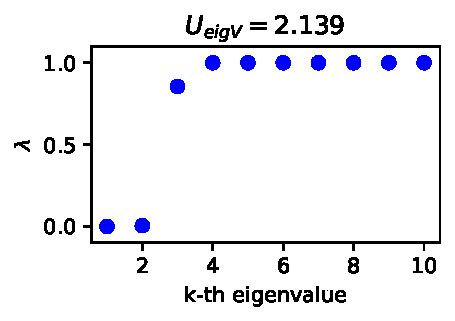
\includegraphics[width=\textwidth]{pics/trivia_low_uq_18_llama.pdf}
    \end{minipage}%\hfill
    \begin{minipage}{0.175\textwidth}
    {\scriptsize
        \begin{verbatim}
 Pink Floyd
 Pink Floyd in Edinburgh
 Pink Floyd
 Shambles
 Pink Floyd
 Pink Floyd
 Pink Floyd
 Pink Floyd
 Pink Floyd
 Pink Floyd
        \end{verbatim} %Dave Gilmore and Roger Waters were in which rock group? Pink Floyd
        }
    \end{minipage}\hspace{10mm}
    \begin{minipage}{0.27\textwidth}
        \centering
        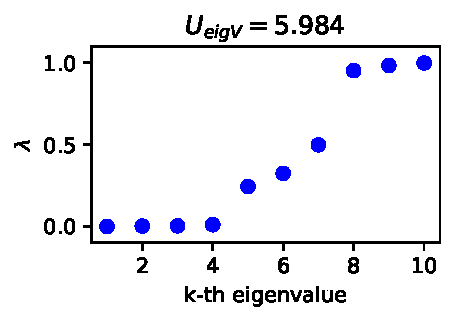
\includegraphics[width=\textwidth]{pics/trivia_high_uq_4_llama.pdf}
    \end{minipage}%\hfill
    \begin{minipage}{0.17\textwidth}
    {\scriptsize
        \begin{verbatim}
 Leukemia
 Low Blood Pressure
 Cervical cancer
 Cancer in 1953 at 41
 Breast cancer
 Tuberculosis
 Cancer
 Leukaemia
 Cancer (in 1953 at age 41)
 Throat cancer
        \end{verbatim} %What claimed the life of singer Kathleen Ferrier? Cancer
        }
    \end{minipage}
    }
    \caption{The distribution of the eigenvalues of the graph Laplacian generated by $\affinityEntail$, for two questions from \datasettrivia,  as well as the 10 generated responses.
    On the left, the question and reference answer are ``Q: Dave Gilmore and Roger Waters were in which rock group? A: Pink Floyd''.
    We have somewhere between two and three meanings, and $U_{\methodEigvClip}$ is slightly above 2. 
    The question on the right is ``Q: What claimed the life of singer Kathleen Ferrier? A: Cancer'', and we observe more diverse responses. %, some of which are spelled differently but have similar/the same meanings. 
    As a result, we see a higher $U_{\methodEigvClip}$ (almost 6).
    }
    \label{fig:eigv}
\end{figure}




\textbf{The Degree Matrix}
The previous two methods helped us define the uncertainty $U(x)$ but cannot assign a confidence score to each generated response.
We utilize the degree matrix $D$ in \cref{eq:D} to define both metrics, as  $D$ already contains relevant information: A node with high degree is well-connected to other nodes, suggesting that it lies in a confident region of the LLM. 
We thus define uncertainty estimate $U_{\methodDegree}(x)$ and confidence score $C_{\methodDegree}(x, \mathbf{s}_j) $ as
\begin{align}
    &U_{\methodDegree}(x) = trace(mI-D)/m^2
    &C_{\methodDegree}(x, \mathbf{s}_j) = D_{j,j}/m.
\end{align}
Here, we assume $W_{j_1,j_2}\in[0,1]$.
$U_{\methodDegree}$ can also be interpreted as the average pairwise distance. 


\textbf{Eccentricity}
Recall that one challenge from earlier is that we only have the similarity (or distance) between different responses, but do not know their actual embedding space.
The graph Laplacian, however, can provide us with coordinates for the responses.
Denote $\mathbf{u}_1, \ldots, \mathbf{u}_k\in\mathbb{R}^m$ as the smallest $k$ eigenvectors of $L$, then an informative embedding of $\mathbf{s}_j$ is simply $\mathbf{v}_j = [u_{1,j},\ldots,u_{k,j}]$~\citep{NIPS2001_801272ee,von2007tutorial}.
As a result, we could use the average distance from center as the uncertainty measure, and each response's distance from the center as the (negative) confidence. 
Formally, the ``eccentricity'' estimates are:
\begin{align}
    & U_{\methodEcc}(x) = \|[\mathbf{v}^{'\top}_1, \ldots, \mathbf{v}^{'\top}_m]\|_2 
    & C_{\methodEcc}(x, \mathbf{s}_j) = -\|\mathbf{v}'_j\|_2
\end{align}
where $\mathbf{v}'_j = \mathbf{v}_j - \frac{1}{m}\sum_{j'=1}^m \mathbf{v}_{j'}$ represents the offset from the average embedding.
\cite{ren2023outofdistribution} uses a similar idea for OOD detection for LLMs, which however requires white-box access to the original language model.
\cref{fig:embed} illustrates a sample embedding (from \datasetcoqa).

\textbf{Remark:}
The confidence scores $C_{\methodEcc}$ and $C_{\methodDegree}$ in the current form are hardly interpretable.
For example, $C_{\methodEcc}$ could have a value of 10 or 0.4.
In practice, they could easily be \textit{calibrated} to match the probability of whether the answer is correct.
In \cref{appendix:calib} we show that with simple calibration these confidence scores could faithfully reflect the probability of correct answer.

\def \FigEmbedding{
\begin{wrapfigure}[18]{R}{0.5\textwidth}
\centering
\vspace{-4mm}
  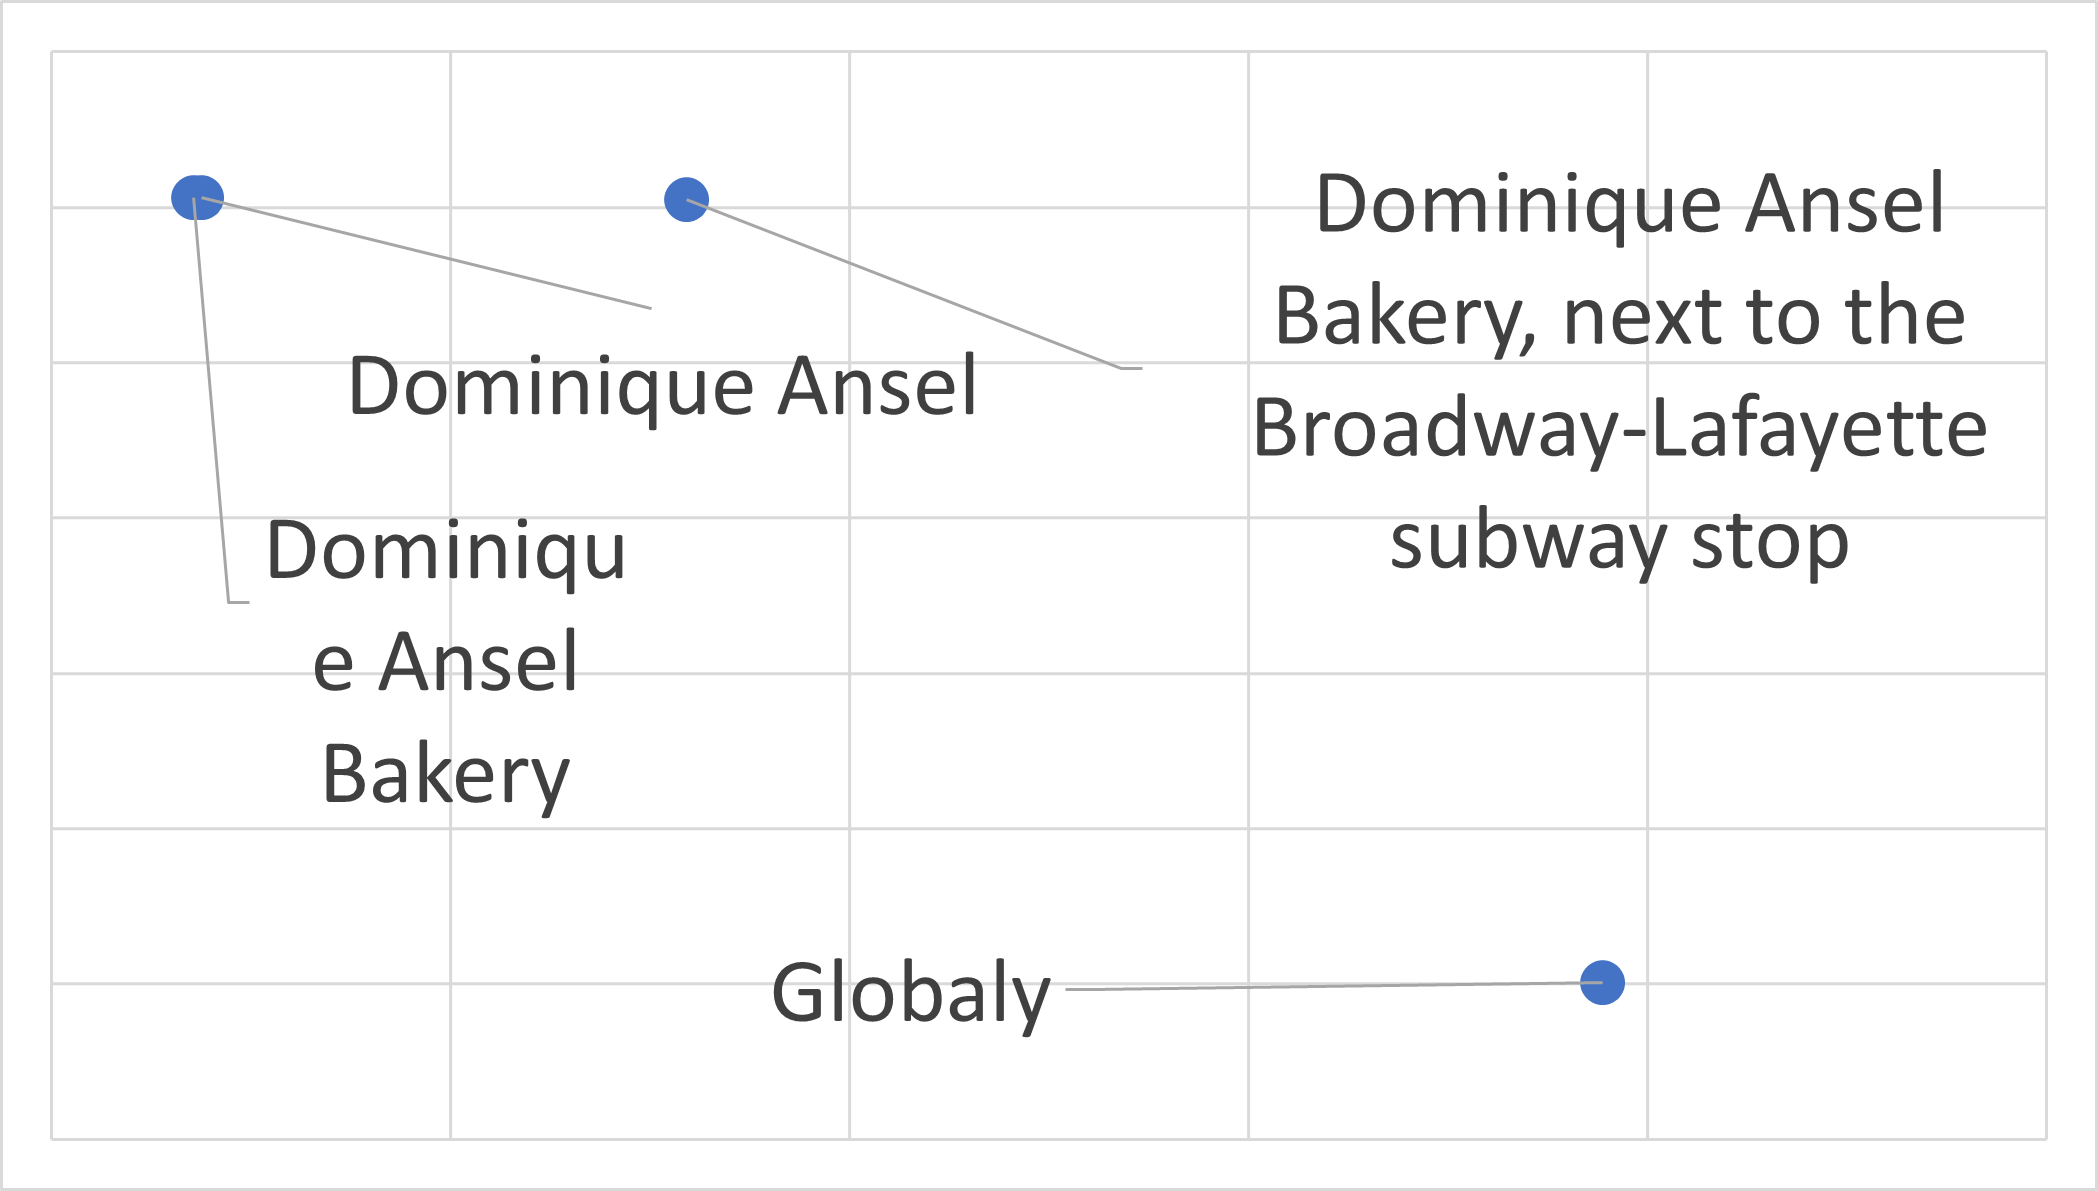
\includegraphics[width=1\textwidth]{pics/embedding.png} 
  \caption{
  An example of the 2D UMAP~\citep{2018arXivUMAP} projection of the embeddings used in \methodEcc for 20 responses. 
  The question and answer are ``Q: What is the bakery's name? A:the Dominique Ansel Bakery''.
  Similar answers tend to live closely together, justifying the use of distance-based uncertainty and confidence measures ($U_\methodEcc$ and $C_\methodEcc$).
  }\label{fig:embed}
\end{wrapfigure}
}
\FigEmbedding